\section{Resultados}

\begin{figure}[H]
\begin{center}
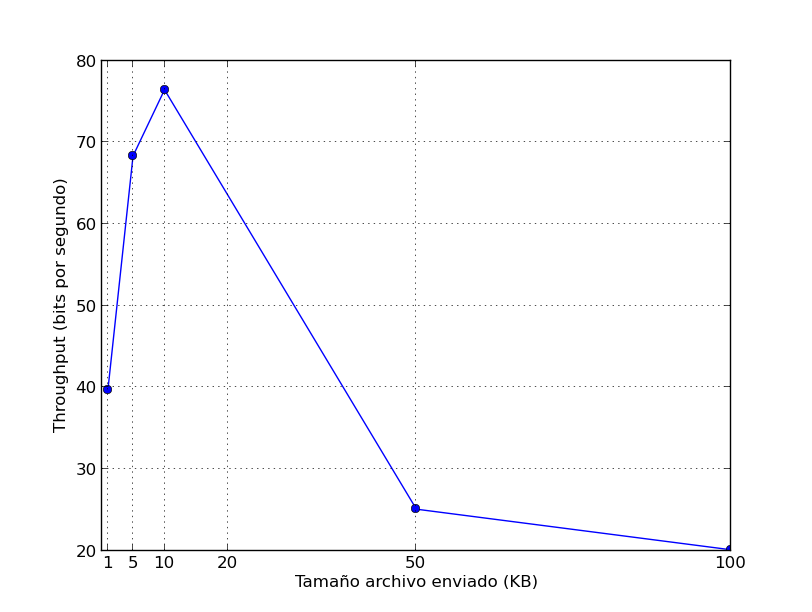
\includegraphics[width=\textwidth,keepaspectratio]{throughput.png}
\end{center}
\caption{Throughput percibido (ventana de emisión fija en 10)} \label{figura1}
\end{figure}

\begin{figure}[H]
\begin{center}
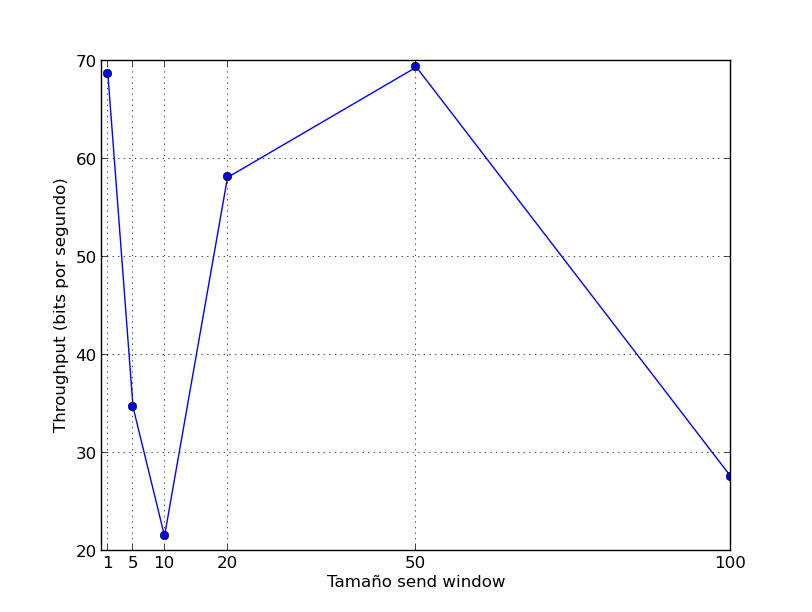
\includegraphics[width=\textwidth,keepaspectratio]{throughput50.png}
\end{center}
\caption{Throughput percibido (tamaño de archivo fijo de 50KB)} \label{figura3}
\end{figure}

%~ \begin{figure}[H]
%~ \begin{center}
%~ 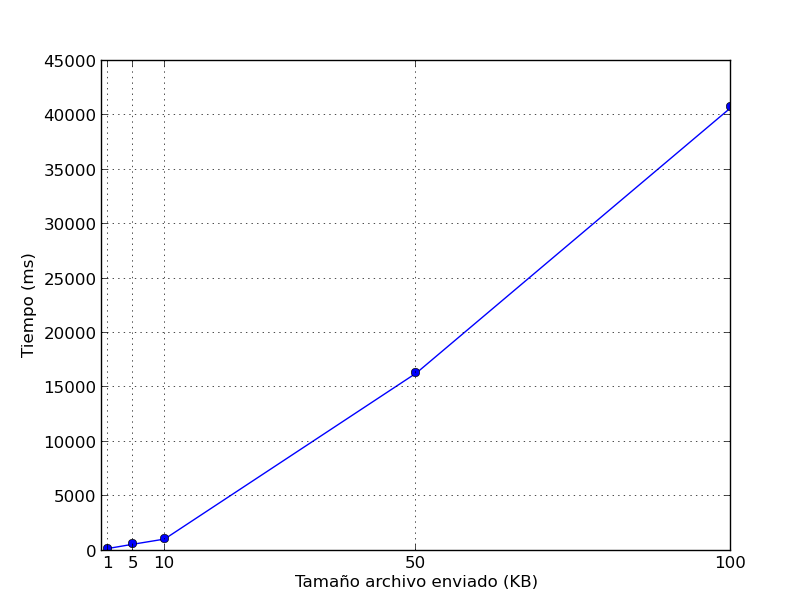
\includegraphics[width=\textwidth,keepaspectratio]{tiempos.png}
%~ \end{center}
%~ \caption{Tiempo total de transmición (ventana de emisión fija en 10)} \label{figura3}
%~ \end{figure}
%~ 
%~ 
%~ \begin{figure}[H]
%~ \begin{center}
%~ 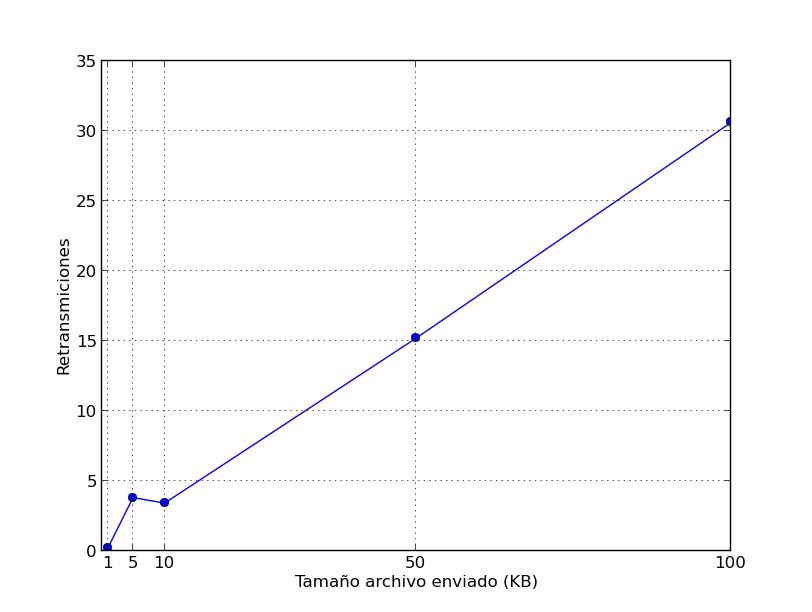
\includegraphics[width=\textwidth,keepaspectratio]{retransmiciones.png}
%~ \end{center}
%~ \caption{Cantidad de retransmiciones (ventana de emisión fija en 10)} \label{figura4}
%~ \end{figure}
%~ 
%~ 
%~ \begin{figure}[H]
%~ \begin{center}
%~ 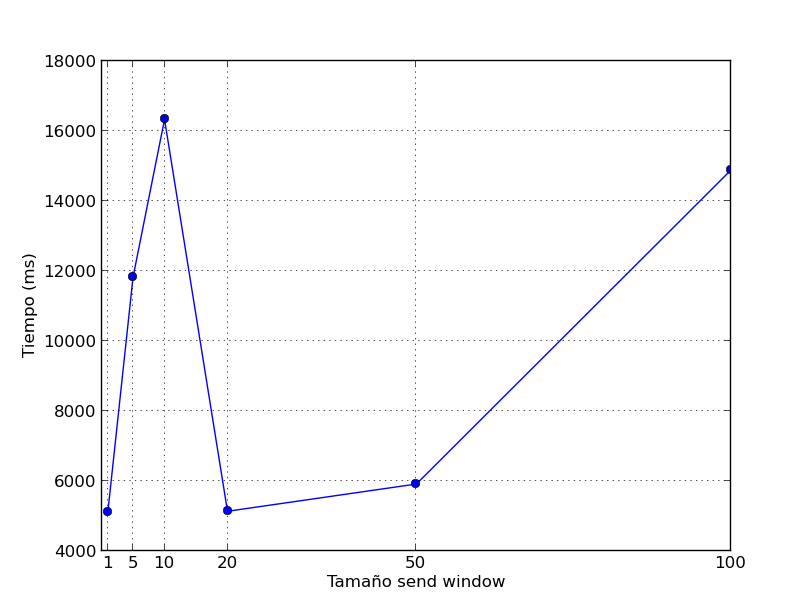
\includegraphics[width=\textwidth,keepaspectratio]{tiempos50.png}
%~ \end{center}
%~ \caption{Tiempo total de transmición (tamaño de archivo fijo de 50KB)} \label{figura5}
%~ \end{figure}

\begin{figure}[H]
\begin{center}
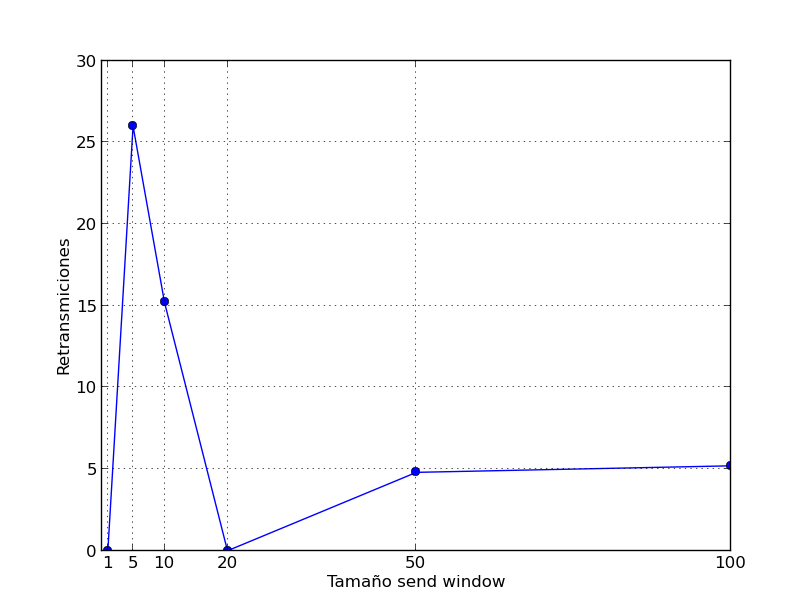
\includegraphics[width=\textwidth,keepaspectratio]{retransmiciones50.png}
\end{center}
\caption{Cantidad de retransmiciones (tamaño de archivo fijo de 50KB)} \label{figura6}
\end{figure}

\begin{figure}[H]
\begin{center}
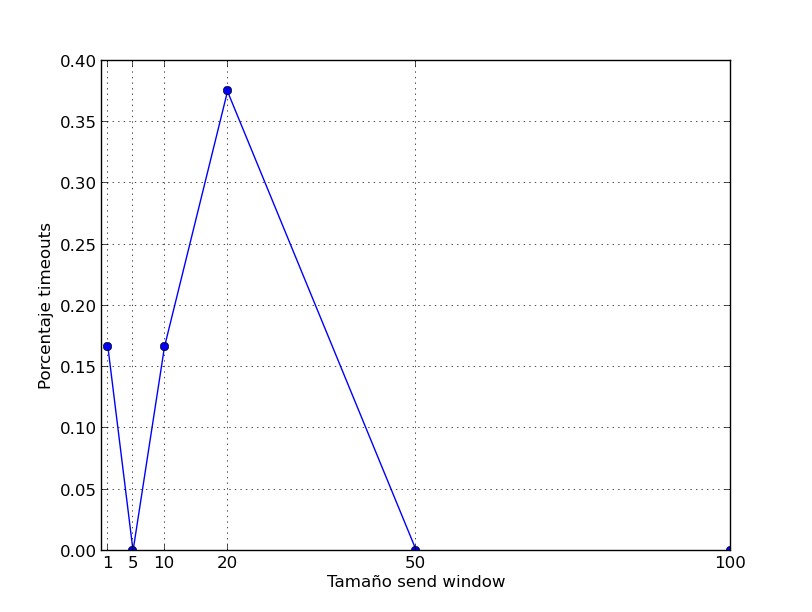
\includegraphics[width=\textwidth,keepaspectratio]{porcentajetimeouts50.png}
\end{center}
\caption{Porcentaje de timeouts por muchas retransmiciones (tamaño de archivo fijo de 50KB)} \label{figura7}
\end{figure}
